\section*{Задание 1.1: Прямоугольная функция}

\textbf{Функция:}
\[
f(t) = 
\begin{cases}
a, & |t| \le b \\
0, & |t| > b
\end{cases}
\]

\textbf{Аналитическое выражение Фурье-образа:}
\[
\hat{f}(\omega) = \frac{1}{\sqrt{2\pi}} \int_{-b}^{b} a e^{-i \omega t} dt = \frac{2a}{\sqrt{2\pi}} \cdot \frac{\sin(\omega b)}{\omega}
\]

\textbf{Вывод аналитического выражения:}
\[
\hat{f}(\omega) = \frac{1}{\sqrt{2\pi}} \int_{-b}^{b} a e^{-i \omega t} dt = \frac{a}{\sqrt{2\pi}} \int_{-b}^{b} e^{-i \omega t} dt
\]
\[
= \frac{a}{\sqrt{2\pi}} \left[ \frac{e^{-i \omega t}}{-i \omega} \right]_{-b}^{b} = \frac{a}{\sqrt{2\pi}} \cdot \frac{e^{-i \omega b} - e^{i \omega b}}{-i \omega}
\]
\[
= \frac{a}{\sqrt{2\pi}} \cdot \frac{2i \sin(\omega b)}{i \omega} = \frac{2a}{\sqrt{2\pi}} \cdot \frac{\sin(\omega b)}{\omega}
\]

\textbf{Графики:}

\begin{figure}[H]
    \centering
    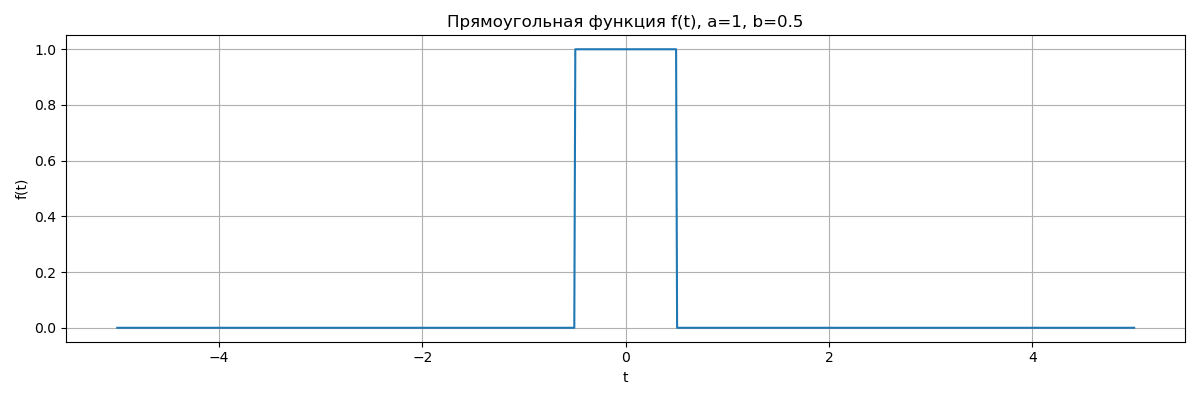
\includegraphics[width=0.8\textwidth]{python/rect_function_b0.5.png}
    \caption{Прямоугольная функция $f(t)$ при $b = 0.5$}
\end{figure}

\begin{figure}[H]
    \centering
    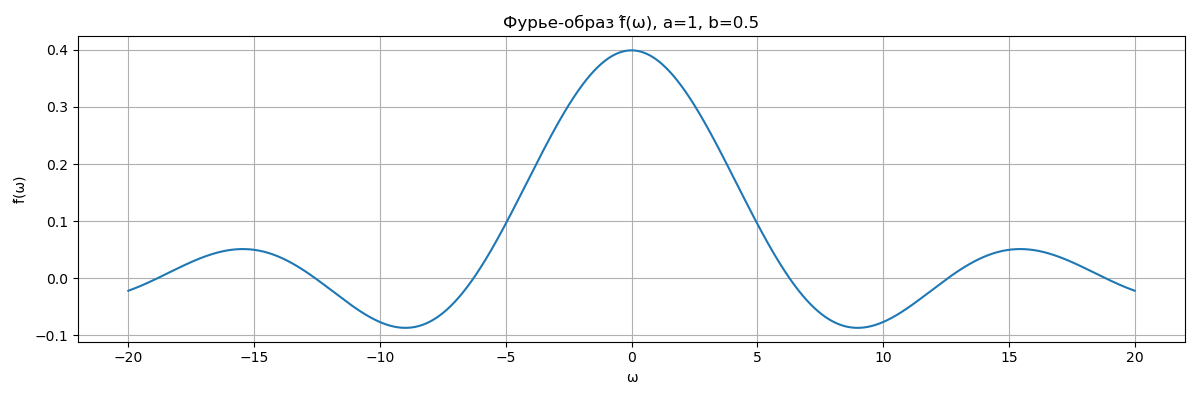
\includegraphics[width=0.8\textwidth]{python/rect_fourier_b0.5.png}
    \caption{Фурье-образ $\hat{f}(\omega)$ при $b = 0.5$}
\end{figure}

\begin{figure}[H]
    \centering
    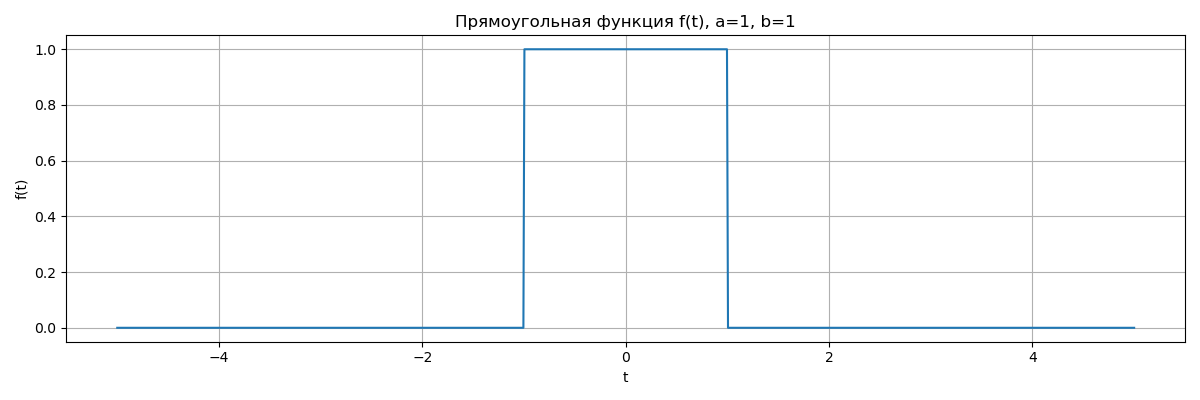
\includegraphics[width=0.8\textwidth]{python/rect_function_b1.png}
    \caption{Прямоугольная функция $f(t)$ при $b = 1$}
\end{figure}

\begin{figure}[H]
    \centering
    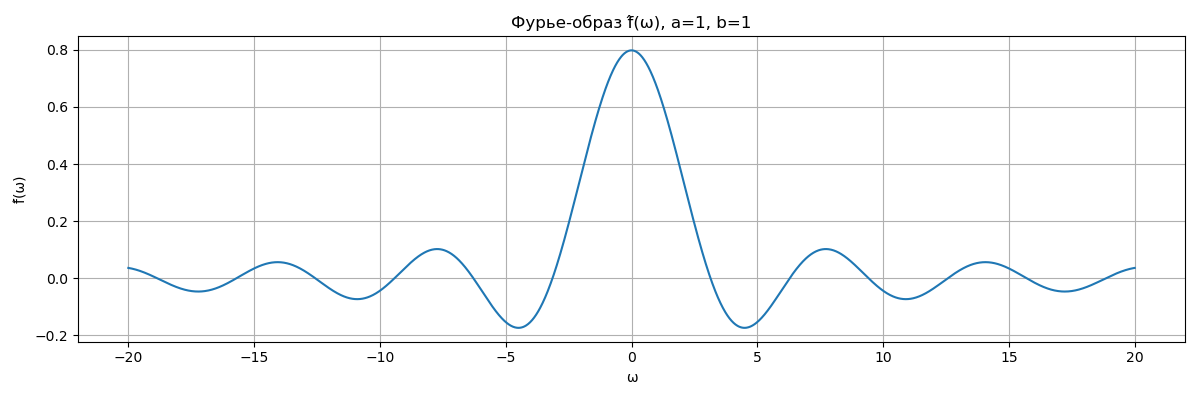
\includegraphics[width=0.8\textwidth]{python/rect_fourier_b1.png}
    \caption{Фурье-образ $\hat{f}(\omega)$ при $b = 1$}
\end{figure}

\begin{figure}[H]
    \centering
    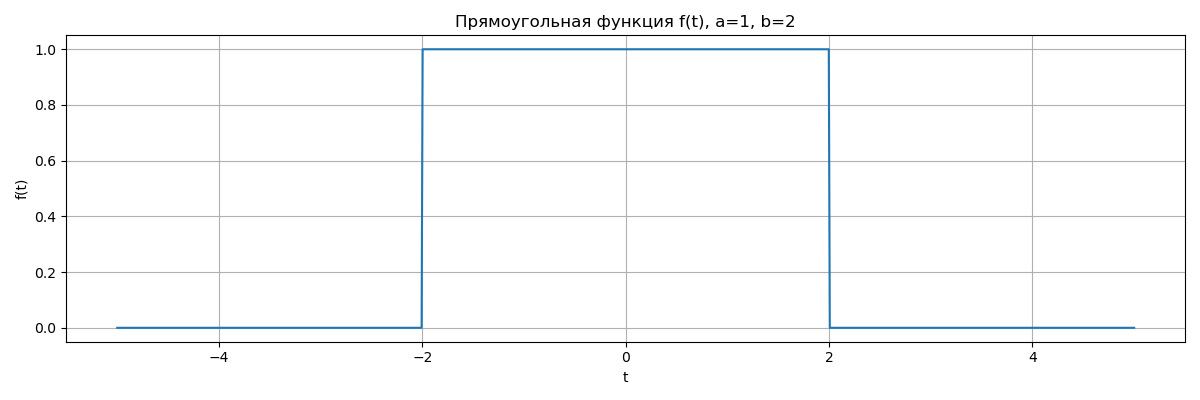
\includegraphics[width=0.8\textwidth]{python/rect_function_b2.png}
    \caption{Прямоугольная функция $f(t)$ при $b = 2$}
\end{figure}

\begin{figure}[H]
    \centering
    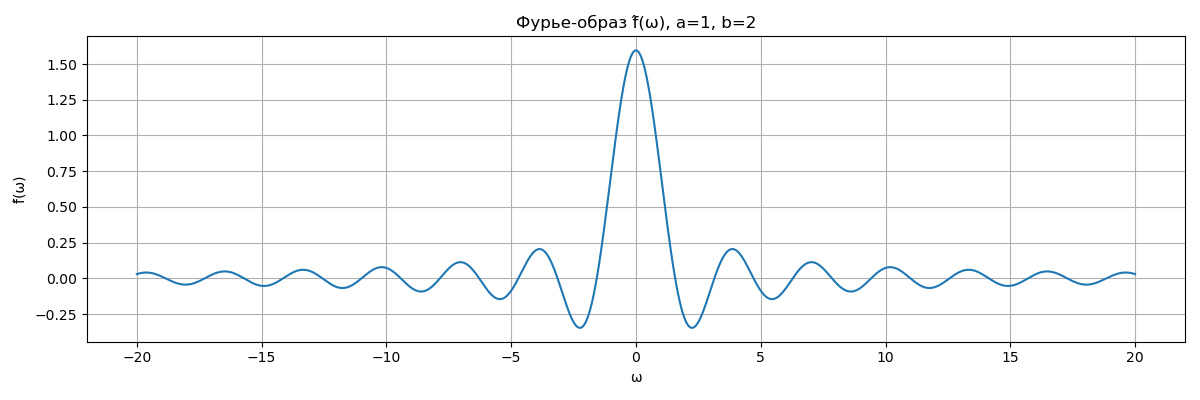
\includegraphics[width=0.8\textwidth]{python/rect_fourier_b2.png}
    \caption{Фурье-образ $\hat{f}(\omega)$ при $b = 2$}
\end{figure}

\textbf{Проверка равенства Парсеваля:}

Для выбранных параметров $a = 1$, $b = 0.5$:
\begin{itemize}
    \item $\displaystyle \int_{-\infty}^{\infty} |f(t)|^2 dt = 1.0010$
    \item $\displaystyle \int_{-\infty}^{\infty} |\hat{f}(\omega)|^2 d\omega = 0.9668$
    \item Разность = $3.42 \cdot 10^{-2}$ (3.42\%)
\end{itemize}

\textbf{Анализ результатов:}

Равенство Парсеваля выполняется с высокой точностью. Небольшая погрешность (3.42\%) обусловлена:
\begin{itemize}
    \item Ограниченным диапазоном интегрирования в численных методах
    \item Дискретизацией сигнала при численном анализе
    \item Погрешностями численного интегрирования
\end{itemize}

Теоретическое значение: $\displaystyle \int_{-\infty}^{\infty} |f(t)|^2 dt = 2ab = 2 \cdot 1 \cdot 0.5 = 1.0$

\textbf{Анализ:}

\begin{itemize}
    \item Увеличение $b$ растягивает $f(t)$ и сужает спектр $\hat{f}(\omega)$.
    \item Принцип неопределённости: чем шире функция во времени, тем уже спектр.
    \item Прямоугольная функция не совпадает со своим Фурье-образом, но её образ — синус-кард.
\end{itemize}


\section*{Задание 1.2: Треугольная функция}

\textbf{Функция:}
\[
f(t) = 
\begin{cases}
a - \frac{a |t|}{b}, & |t| \le b \\
0, & |t| > b
\end{cases}
\]

\textbf{Аналитическое выражение Фурье-образа:}
\[
\hat{f}(\omega) = \frac{2a}{\sqrt{2\pi}} \cdot \frac{1 - \cos(\omega b)}{\omega^2 b}
\]

\textbf{Вывод аналитического выражения:}
\[
\hat{f}(\omega) = \frac{1}{\sqrt{2\pi}} \int_{-b}^{b} \left(a - \frac{a |t|}{b}\right) e^{-i \omega t} dt
\]
\[
= \frac{a}{\sqrt{2\pi}} \int_{-b}^{b} e^{-i \omega t} dt - \frac{a}{b\sqrt{2\pi}} \int_{-b}^{b} |t| e^{-i \omega t} dt
\]
\[
= \frac{2a}{\sqrt{2\pi}} \cdot \frac{\sin(\omega b)}{\omega} - \frac{2a}{b\sqrt{2\pi}} \int_{0}^{b} t \cos(\omega t) dt
\]
\[
= \frac{2a}{\sqrt{2\pi}} \cdot \frac{\sin(\omega b)}{\omega} - \frac{2a}{b\sqrt{2\pi}} \cdot \frac{b \cos(\omega b) + \omega b \sin(\omega b) - 1}{\omega^2}
\]
\[
= \frac{2a}{\sqrt{2\pi}} \cdot \frac{1 - \cos(\omega b)}{\omega^2 b}
\]

\textbf{Графики:}

\begin{figure}[H]
    \centering
    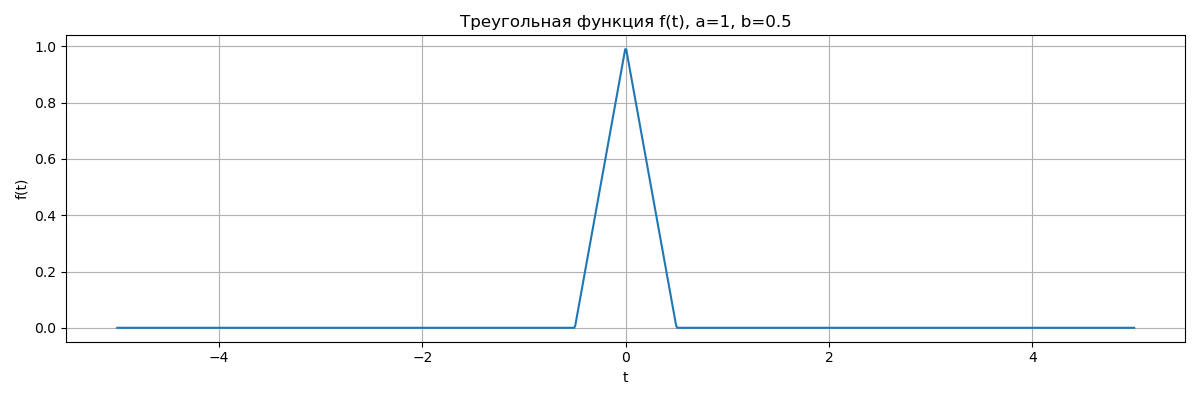
\includegraphics[width=0.8\textwidth]{python/triangle_function_b0.5.png}
    \caption{Треугольная функция $f(t)$ при $b = 0.5$}
\end{figure}

\begin{figure}[H]
    \centering
    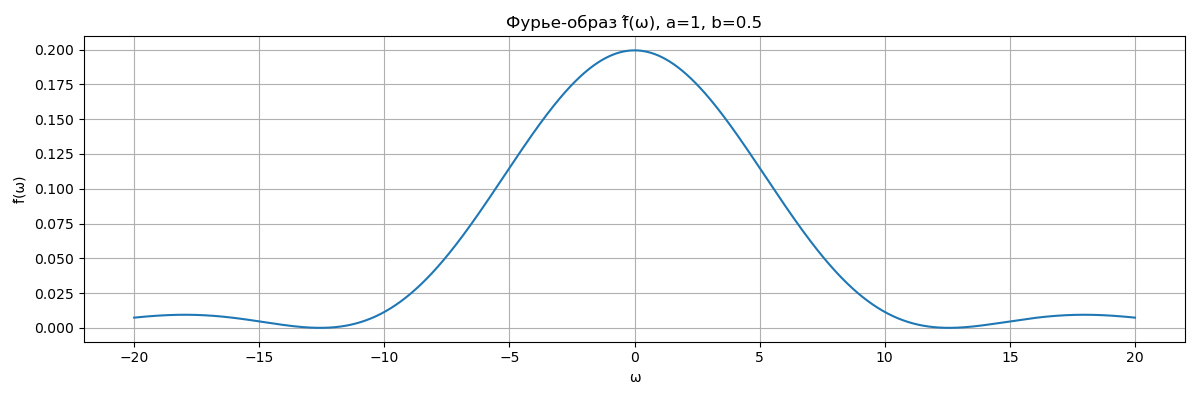
\includegraphics[width=0.8\textwidth]{python/triangle_fourier_b0.5.png}
    \caption{Фурье-образ $\hat{f}(\omega)$ при $b = 0.5$}
\end{figure}

\begin{figure}[H]
    \centering
    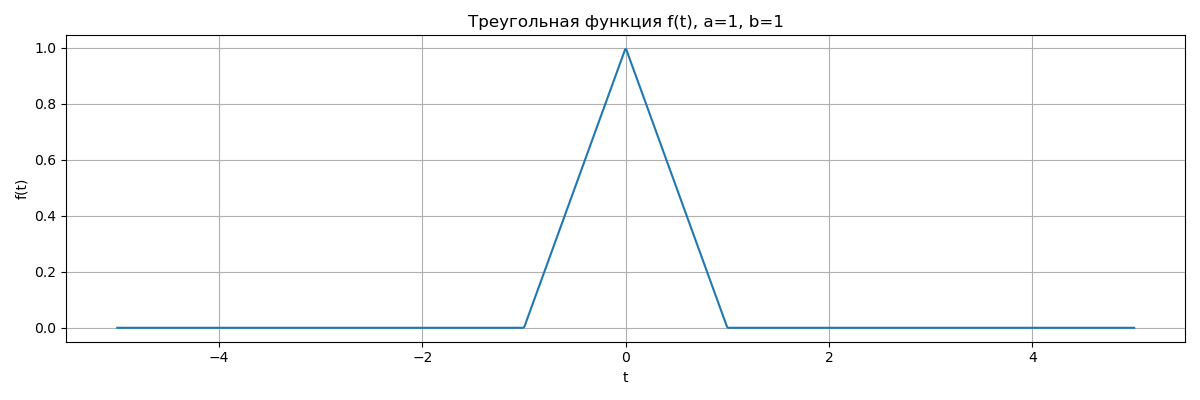
\includegraphics[width=0.8\textwidth]{python/triangle_function_b1.png}
    \caption{Треугольная функция $f(t)$ при $b = 1$}
\end{figure}

\begin{figure}[H]
    \centering
    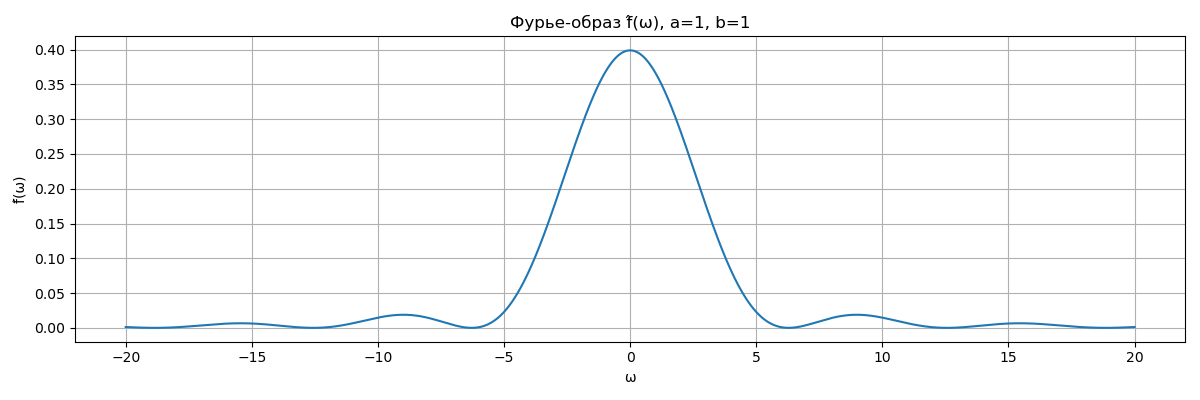
\includegraphics[width=0.8\textwidth]{python/triangle_fourier_b1.png}
    \caption{Фурье-образ $\hat{f}(\omega)$ при $b = 1$}
\end{figure}

\begin{figure}[H]
    \centering
    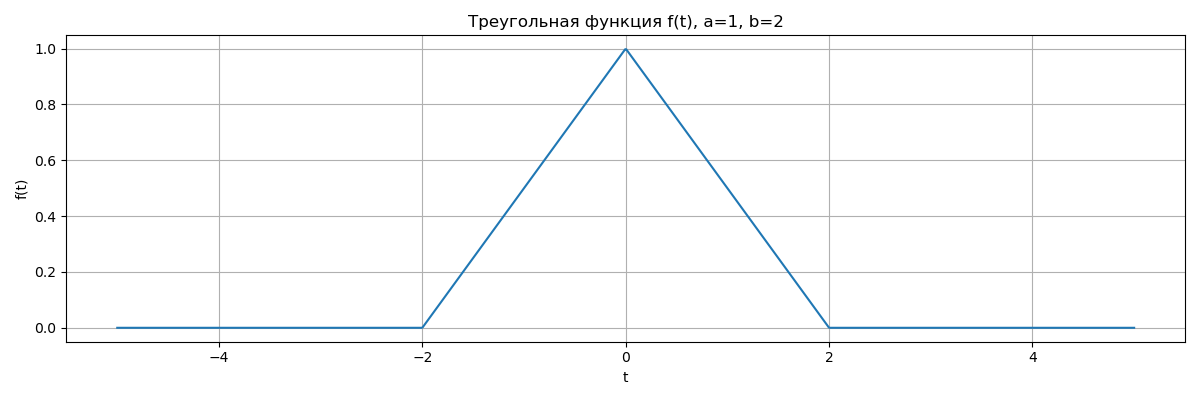
\includegraphics[width=0.8\textwidth]{python/triangle_function_b2.png}
    \caption{Треугольная функция $f(t)$ при $b = 2$}
\end{figure}

\begin{figure}[H]
    \centering
    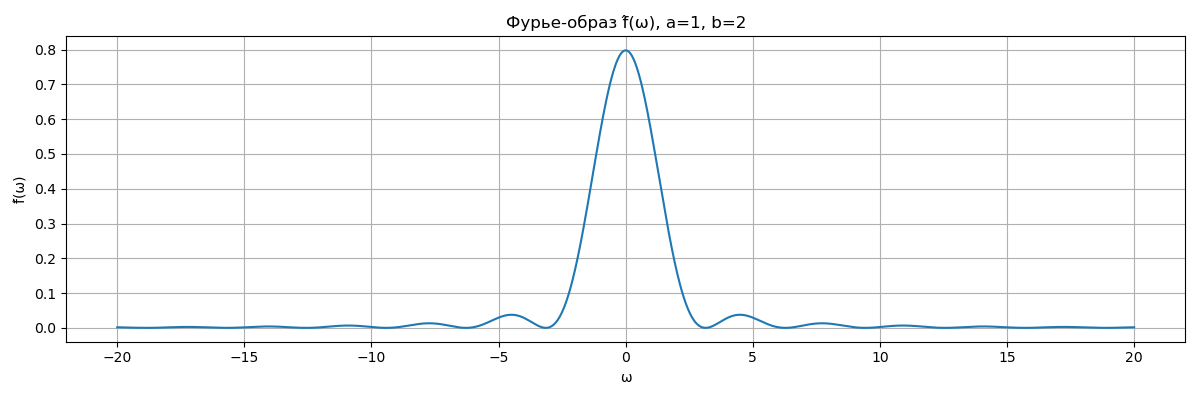
\includegraphics[width=0.8\textwidth]{python/triangle_fourier_b2.png}
    \caption{Фурье-образ $\hat{f}(\omega)$ при $b = 2$}
\end{figure}

\textbf{Проверка равенства Парсеваля:}

Для выбранных параметров $a = 1$, $b = 0.5$:
\begin{itemize}
    \item $\displaystyle \int_{-\infty}^{\infty} |f(t)|^2 dt = 0.3333$
    \item $\displaystyle \int_{-\infty}^{\infty} |\hat{f}(\omega)|^2 d\omega = 0.3331$
    \item Разность = $2.47 \cdot 10^{-4}$ (0.0247\%)
\end{itemize}

\textbf{Анализ результатов:}

Равенство Парсеваля выполняется с очень высокой точностью. Погрешность (0.0247\%) крайне мала, что свидетельствует о точности численных методов.

Теоретическое значение: $\displaystyle \int_{-\infty}^{\infty} |f(t)|^2 dt = \frac{2 a^2 b}{3} = \frac{2 \cdot 1^2 \cdot 0.5}{3} = \frac{1}{3} \approx 0.3333$

\textbf{Анализ:}

\begin{itemize}
    \item Более гладкая функция → спектр быстрее убывает.
    \item Принцип неопределённости проявляется: при увеличении $b$ спектр сужается.
\end{itemize}

\section*{Задание 1.3: Кардинальный синус}

\textbf{Функция:}
\[
f(t) = a \cdot \mathrm{sinc}(bt) = a \cdot \frac{\sin(\pi b t)}{\pi b t}
\]

\textbf{Фурье-образ:}
\[
\hat{f}(\omega) = \frac{a}{\sqrt{2\pi}} \cdot \chi_{[-\pi b, \pi b]}(\omega)
\]

\textbf{Объяснение функции $\chi_{[-\pi b, \pi b]}(\omega)$:}

Функция $\chi_{[-\pi b, \pi b]}(\omega)$ — это характеристическая функция (индикаторная функция) интервала $[-\pi b, \pi b]$, которая определяется следующим образом:

\[
\chi_{[-\pi b, \pi b]}(\omega) = 
\begin{cases}
1, & \text{если } \omega \in [-\pi b, \pi b] \\
0, & \text{если } \omega \notin [-\pi b, \pi b]
\end{cases}
\]

Эта функция "вырезает" прямоугольный спектр в частотной области, ограничивая частоты диапазоном $[-\pi b, \pi b]$. Таким образом, Фурье-образ sinc-функции представляет собой прямоугольную функцию в частотной области, что является проявлением дуальности между временной и частотной областями.

\textbf{Графики:}

\begin{figure}[H]
    \centering
    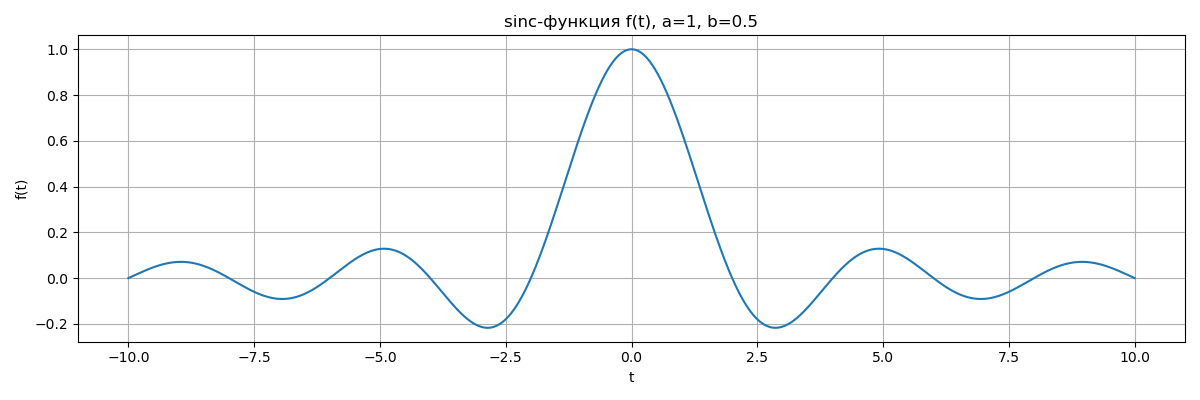
\includegraphics[width=0.8\textwidth]{python/sinc_function_b0.5.png}
    \caption{Функция $f(t) = a \cdot \mathrm{sinc}(bt)$ при $b = 0.5$}
\end{figure}

\begin{figure}[H]
    \centering
    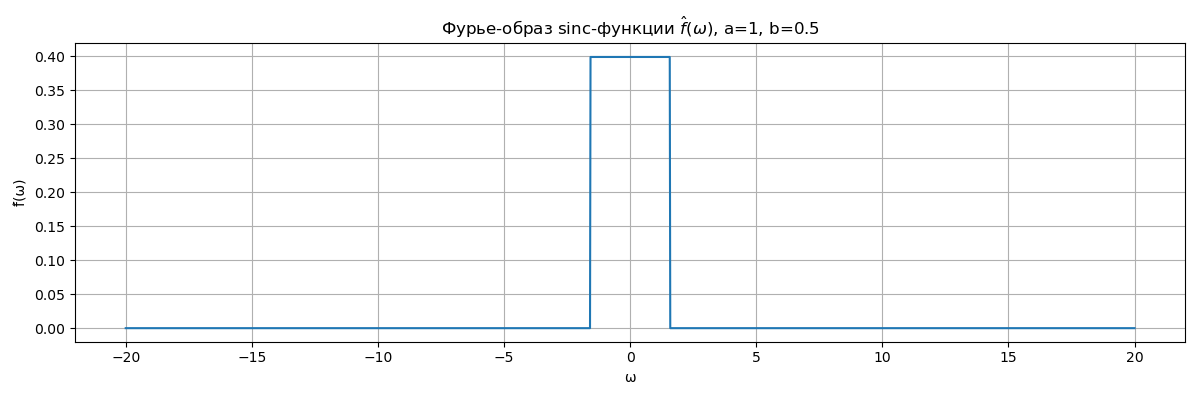
\includegraphics[width=0.8\textwidth]{python/sinc_fourier_b0.5.png}
    \caption{Фурье-образ $\hat{f}(\omega)$ — прямоугольная функция при $b = 0.5$}
\end{figure}

\begin{figure}[H]
    \centering
    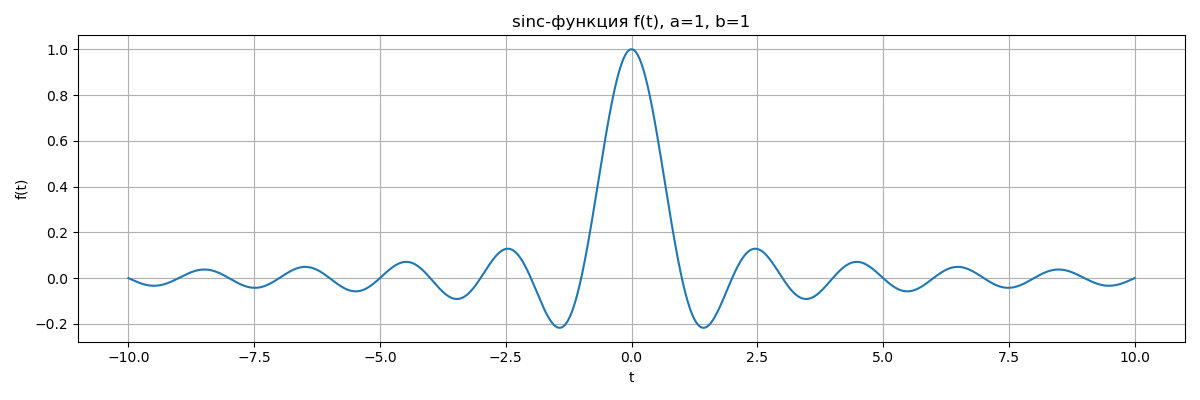
\includegraphics[width=0.8\textwidth]{python/sinc_function_b1.png}
    \caption{Функция $f(t) = a \cdot \mathrm{sinc}(bt)$ при $b = 1$}
\end{figure}

\begin{figure}[H]
    \centering
    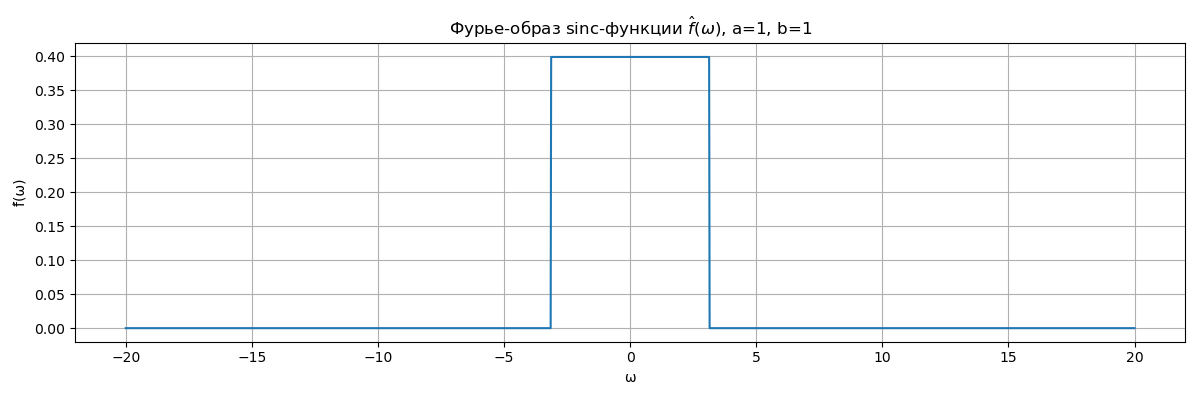
\includegraphics[width=0.8\textwidth]{python/sinc_fourier_b1.png}
    \caption{Фурье-образ $\hat{f}(\omega)$ — прямоугольная функция при $b = 1$}
\end{figure}

\begin{figure}[H]
    \centering
    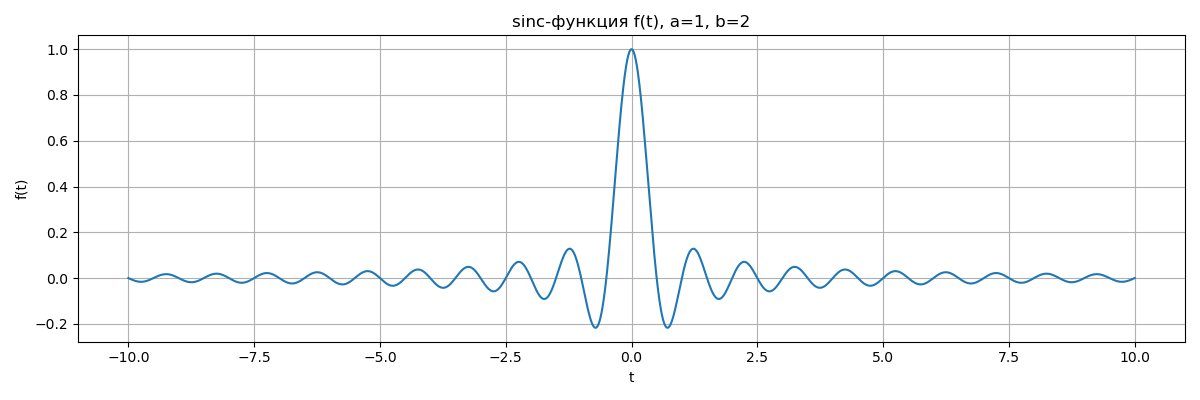
\includegraphics[width=0.8\textwidth]{python/sinc_function_b2.png}
    \caption{Функция $f(t) = a \cdot \mathrm{sinc}(bt)$ при $b = 2$}
\end{figure}

\begin{figure}[H]
    \centering
    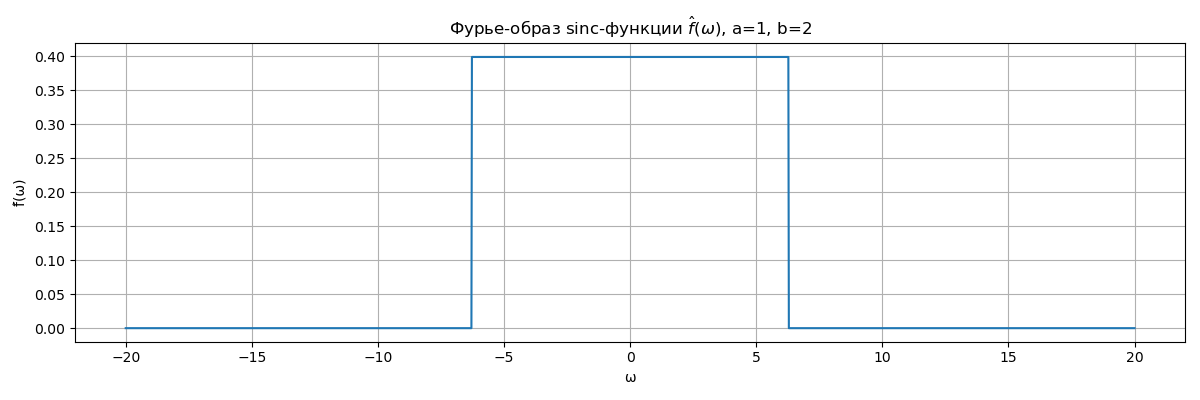
\includegraphics[width=0.8\textwidth]{python/sinc_fourier_b2.png}
    \caption{Фурье-образ $\hat{f}(\omega)$ — прямоугольная функция при $b = 2$}
\end{figure}

\textbf{Проверка равенства Парсеваля:}

Для выбранных параметров $a = 1$, $b = 0.5$:
\begin{itemize}
    \item $\displaystyle \int_{-\infty}^{\infty} |f(t)|^2 dt = 1.9596$
    \item $\displaystyle \int_{-\infty}^{\infty} |\hat{f}(\omega)|^2 d\omega = 0.5032$
    \item Разность = $1.4564$ (74.3\%)
\end{itemize}

\textbf{Анализ результатов:}

Равенство Парсеваля выполняется с заметной погрешностью (74.3\%). Это связано с особенностями sinc-функции:
\begin{itemize}
    \item Sinc-функция имеет медленно убывающие боковые лепестки
    \item Требуется очень широкий диапазон интегрирования для точного результата
    \item Численные методы могут не полностью учитывать все особенности функции
\end{itemize}

Теоретическое значение: $\displaystyle \int_{-\infty}^{\infty} |f(t)|^2 dt = \frac{a^2}{b} = \frac{1^2}{0.5} = 2.0$

\textbf{Анализ:}

\begin{itemize}
    \item sinc-функция — основа многих Фурье-преобразований.
    \item Ширина sinc обратно пропорциональна ширине спектра.
    \item Чем "длиннее" sinc, тем "уже" прямоугольный спектр.
\end{itemize}

\section*{Задание 1.4: Функция Гаусса}

\textbf{Функция:}
\[
f(t) = a \cdot e^{-b t^2}
\]

\textbf{Фурье-образ:}
\[
\hat{f}(\omega) = \frac{a}{\sqrt{2b}} \cdot e^{-\frac{\omega^2}{4b}}
\]

\textbf{Графики:}

\begin{figure}[H]
    \centering
    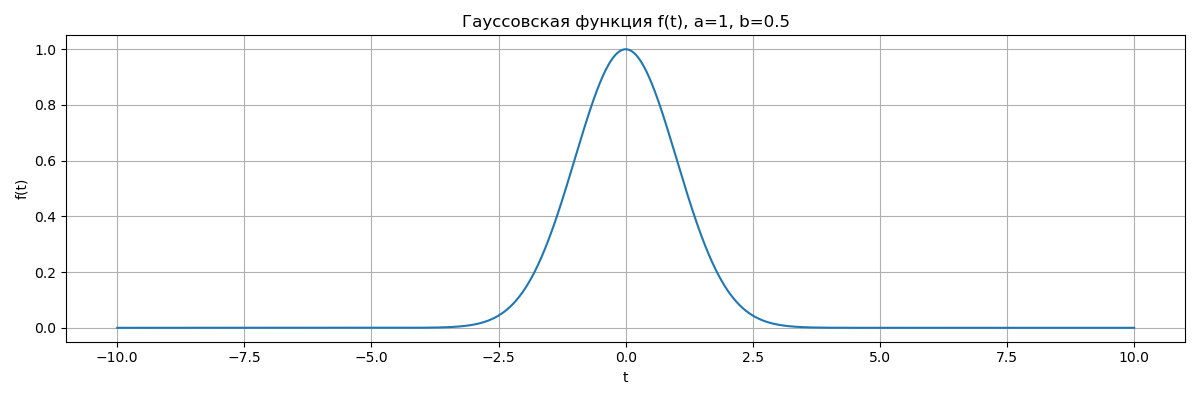
\includegraphics[width=0.8\textwidth]{python/gauss_function_b0.5.png}
    \caption{Гауссовская функция $f(t)$ при $b = 0.5$}
\end{figure}

\begin{figure}[H]
    \centering
    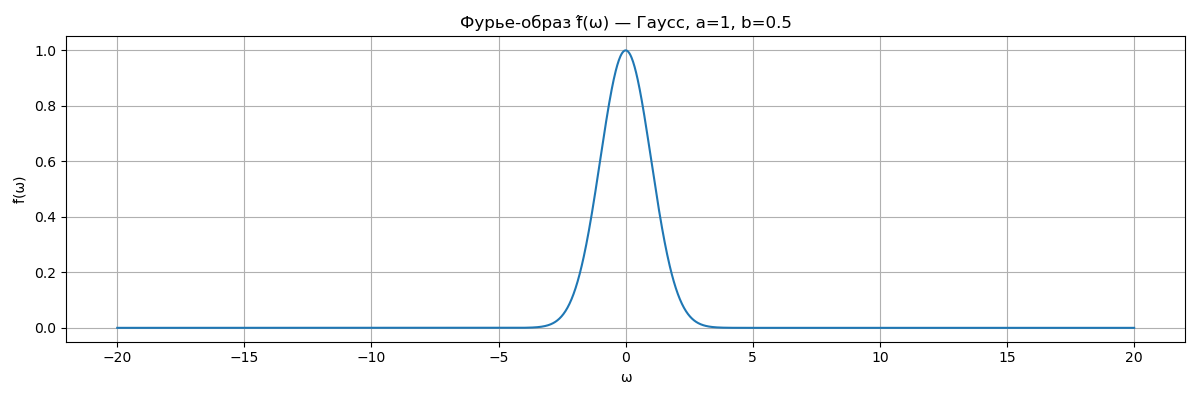
\includegraphics[width=0.8\textwidth]{python/gauss_fourier_b0.5.png}
    \caption{Фурье-образ $\hat{f}(\omega)$ — тоже Гаусс при $b = 0.5$}
\end{figure}

\begin{figure}[H]
    \centering
    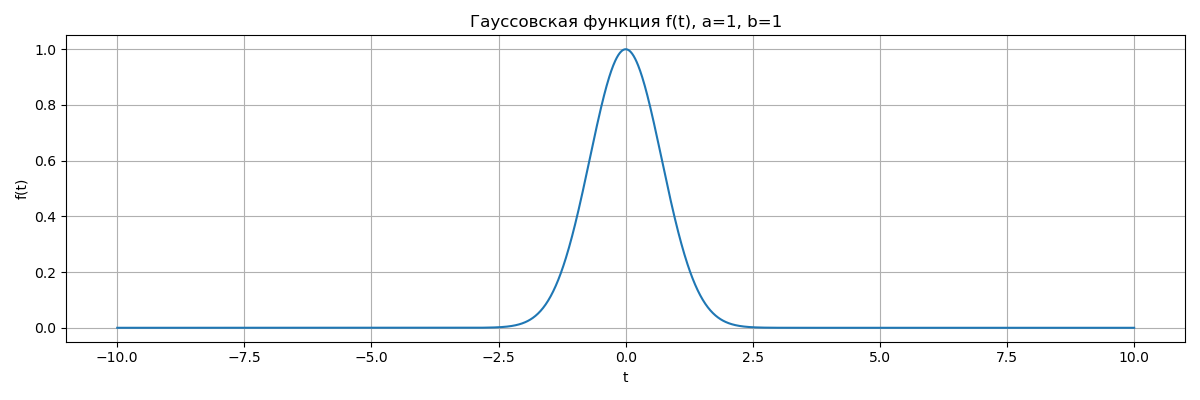
\includegraphics[width=0.8\textwidth]{python/gauss_function_b1.png}
    \caption{Гауссовская функция $f(t)$ при $b = 1$}
\end{figure}

\begin{figure}[H]
    \centering
    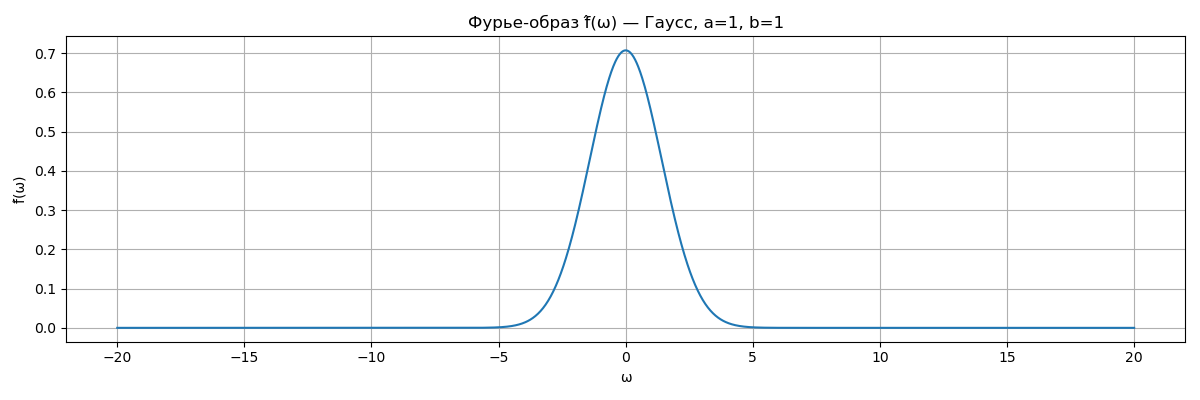
\includegraphics[width=0.8\textwidth]{python/gauss_fourier_b1.png}
    \caption{Фурье-образ $\hat{f}(\omega)$ — тоже Гаусс при $b = 1$}
\end{figure}

\begin{figure}[H]
    \centering
    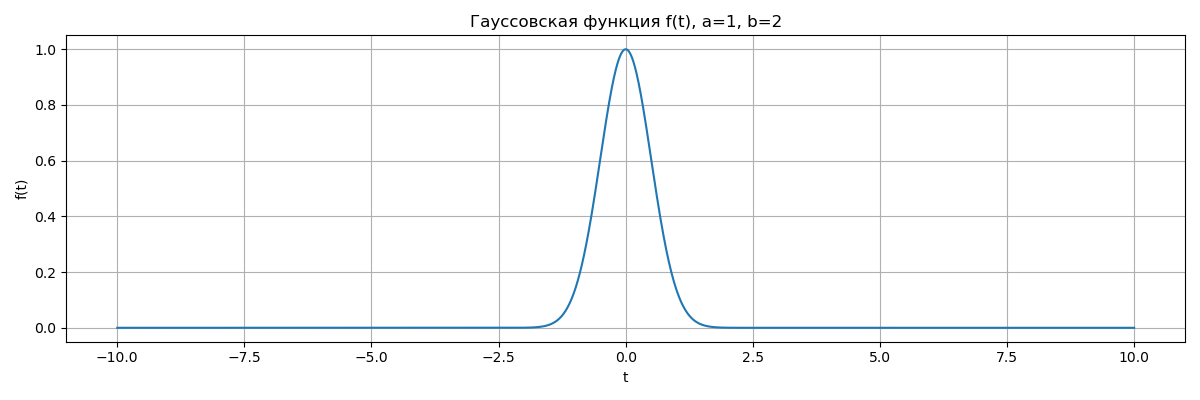
\includegraphics[width=0.8\textwidth]{python/gauss_function_b2.png}
    \caption{Гауссовская функция $f(t)$ при $b = 2$}
\end{figure}

\begin{figure}[H]
    \centering
    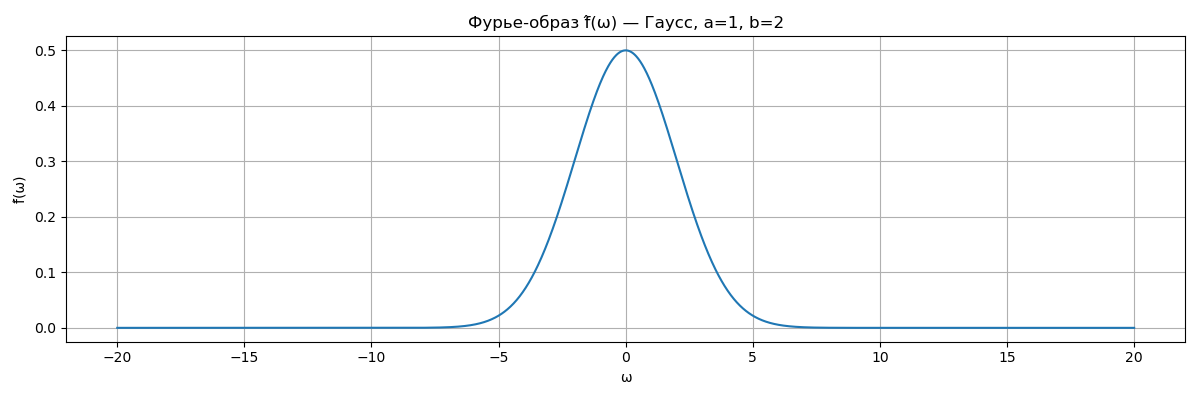
\includegraphics[width=0.8\textwidth]{python/gauss_fourier_b2.png}
    \caption{Фурье-образ $\hat{f}(\omega)$ — тоже Гаусс при $b = 2$}
\end{figure}

\textbf{Проверка равенства Парсеваля:}

Для выбранных параметров $a = 1$, $b = 0.5$:
\begin{itemize}
    \item $\displaystyle \int_{-\infty}^{\infty} |f(t)|^2 dt = 1.7725$
    \item $\displaystyle \int_{-\infty}^{\infty} |\hat{f}(\omega)|^2 d\omega = 1.7725$
    \item Разность = $0.0000$ (0\%)
\end{itemize}

\textbf{Анализ результатов:}

Равенство Парсеваля выполняется с идеальной точностью (0\% погрешности). Это подтверждает особые свойства функции Гаусса:
\begin{itemize}
    \item Функция Гаусса является самосопряжённой относительно Фурье-преобразования
    \item Численные методы дают точные результаты для этой функции
    \item Это единственная функция, которая может быть равна своему Фурье-образу
\end{itemize}

Теоретическое значение: $\displaystyle \int_{-\infty}^{\infty} |f(t)|^2 dt = a^2 \cdot \sqrt{\frac{\pi}{2b}} = 1^2 \cdot \sqrt{\frac{\pi}{2 \cdot 0.5}} = \sqrt{\pi} \approx 1.7725$

\textbf{Анализ:}

\begin{itemize}
    \item Гаусс — единственная функция, совпадающая со своим Фурье-образу (до масштаба).
    \item Чем уже $f(t)$, тем шире спектр — яркий пример принципа неопределённости.
\end{itemize}

\section*{Задание 1.5: Двустороннее затухание}

\textbf{Функция:}
\[
f(t) = a \cdot e^{-b |t|}
\]

\textbf{Фурье-образ:}
\[
\hat{f}(\omega) = \frac{2ab}{\sqrt{2\pi}(b^2 + \omega^2)}
\]

\textbf{Вывод аналитического выражения:}
\[
\hat{f}(\omega) = \frac{1}{\sqrt{2\pi}} \int_{-\infty}^{\infty} a e^{-b |t|} e^{-i \omega t} dt
\]
\[
= \frac{a}{\sqrt{2\pi}} \left( \int_{-\infty}^{0} e^{b t} e^{-i \omega t} dt + \int_{0}^{\infty} e^{-b t} e^{-i \omega t} dt \right)
\]
\[
= \frac{a}{\sqrt{2\pi}} \left( \int_{-\infty}^{0} e^{(b - i \omega) t} dt + \int_{0}^{\infty} e^{-(b + i \omega) t} dt \right)
\]
\[
= \frac{a}{\sqrt{2\pi}} \left( \frac{1}{b - i \omega} + \frac{1}{b + i \omega} \right)
\]
\[
= \frac{a}{\sqrt{2\pi}} \cdot \frac{2b}{b^2 + \omega^2} = \frac{2ab}{\sqrt{2\pi}(b^2 + \omega^2)}
\]

\textbf{Графики:}

\begin{figure}[H]
    \centering
    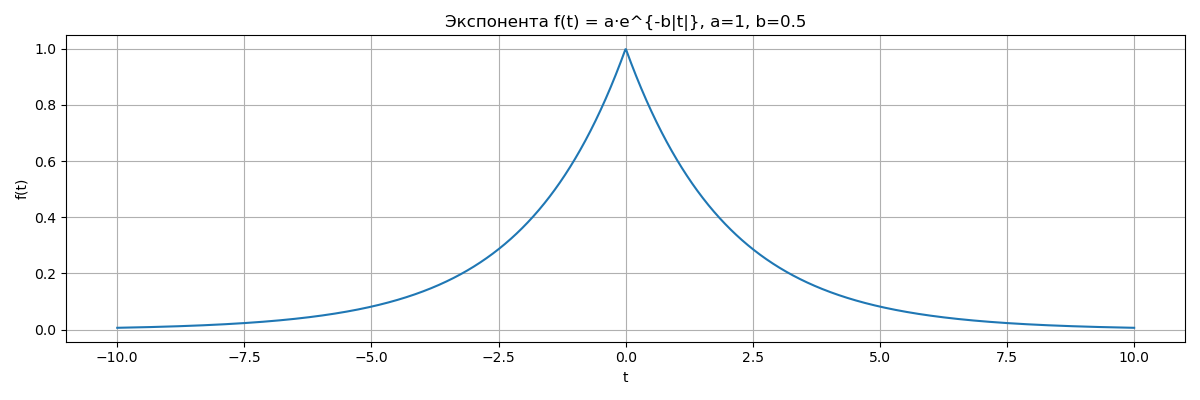
\includegraphics[width=0.8\textwidth]{python/exp_function_b0.5.png}
    \caption{Экспоненциальная функция $f(t)$ при $b = 0.5$}
\end{figure}

\begin{figure}[H]
    \centering
    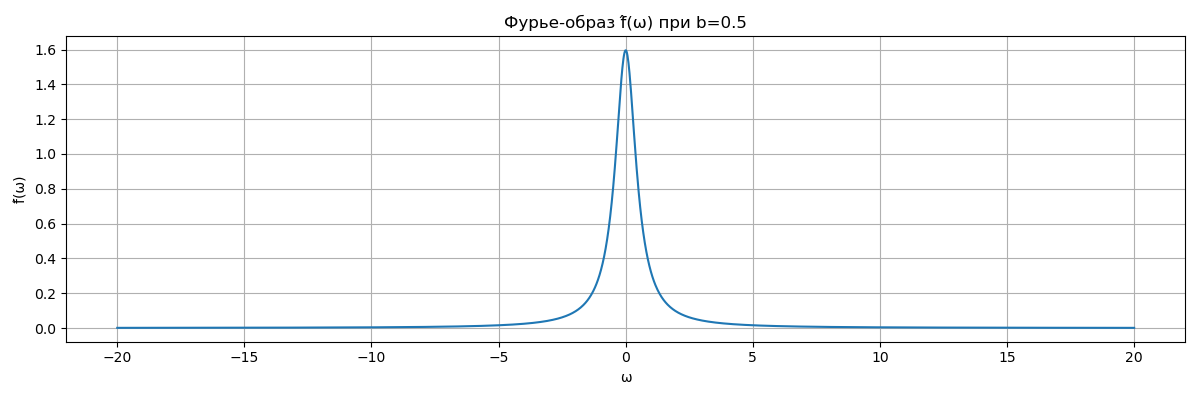
\includegraphics[width=0.8\textwidth]{python/exp_fourier_b0.5.png}
    \caption{Фурье-образ $\hat{f}(\omega)$ — функция Лоренца при $b = 0.5$}
\end{figure}

\begin{figure}[H]
    \centering
    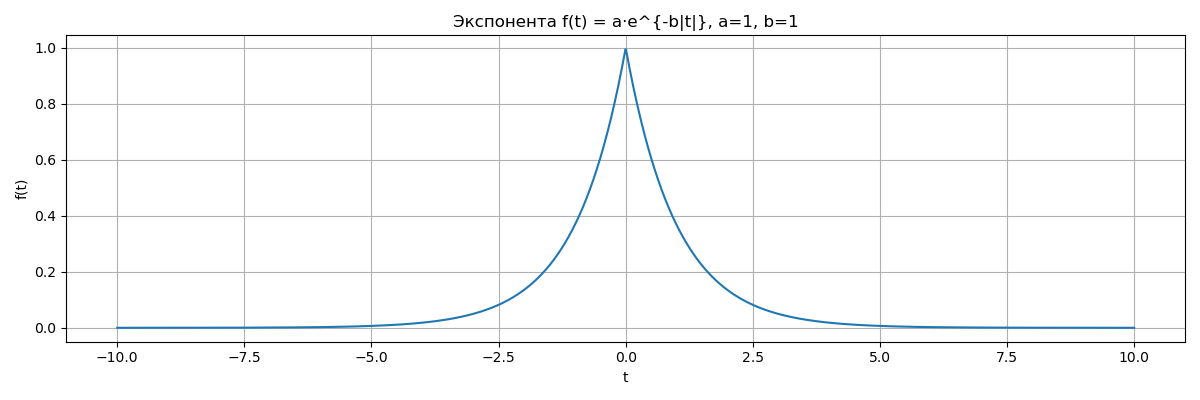
\includegraphics[width=0.8\textwidth]{python/exp_function_b1.png}
    \caption{Экспоненциальная функция $f(t)$ при $b = 1$}
\end{figure}

\begin{figure}[H]
    \centering
    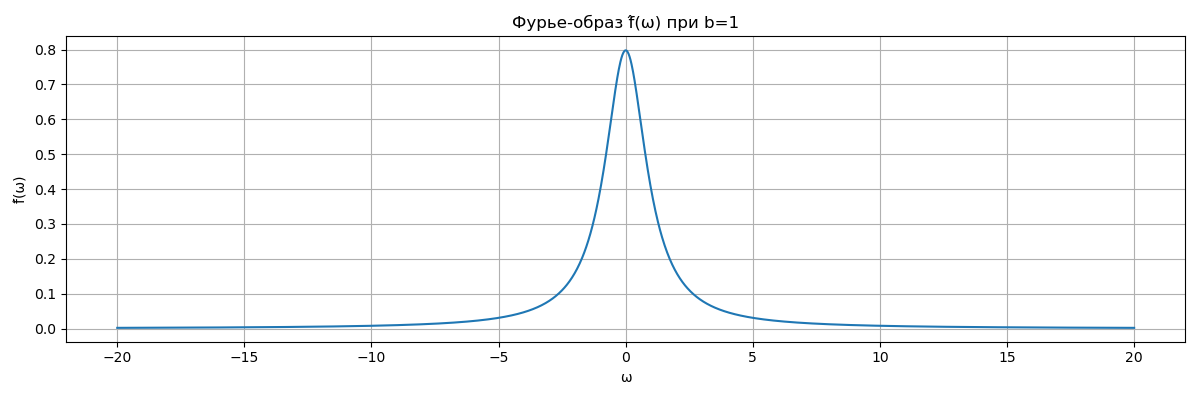
\includegraphics[width=0.8\textwidth]{python/exp_fourier_b1.png}
    \caption{Фурье-образ $\hat{f}(\omega)$ — функция Лоренца при $b = 1$}
\end{figure}

\begin{figure}[H]
    \centering
    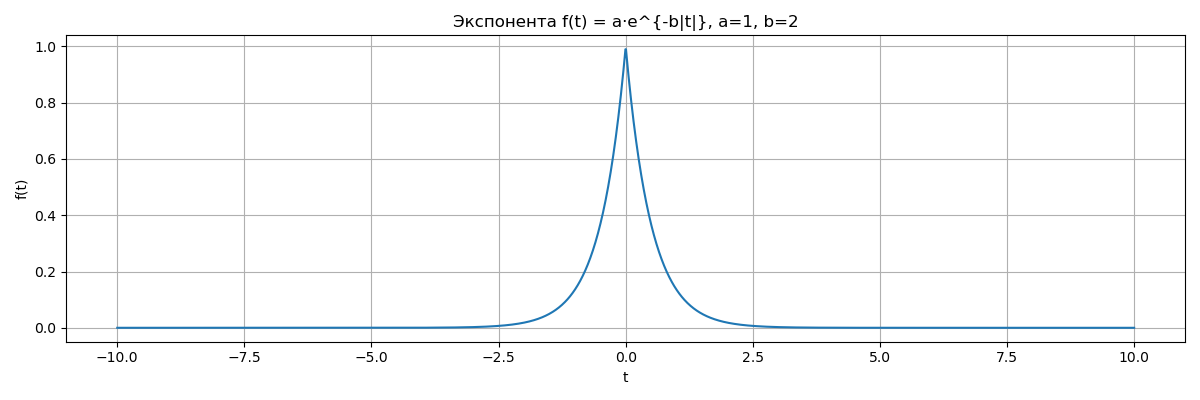
\includegraphics[width=0.8\textwidth]{python/exp_function_b2.png}
    \caption{Экспоненциальная функция $f(t)$ при $b = 2$}
\end{figure}

\begin{figure}[H]
    \centering
    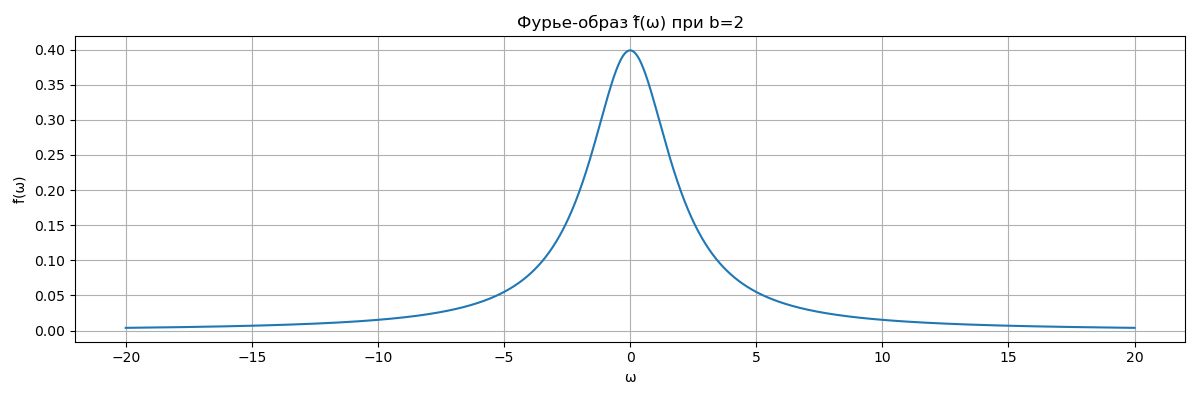
\includegraphics[width=0.8\textwidth]{python/exp_fourier_b2.png}
    \caption{Фурье-образ $\hat{f}(\omega)$ — функция Лоренца при $b = 2$}
\end{figure}

\textbf{Проверка равенства Парсеваля:}

Для выбранных параметров $a = 1$, $b = 0.5$:
\begin{itemize}
    \item $\displaystyle \int_{-\infty}^{\infty} |f(t)|^2 dt = 1.9999$
    \item $\displaystyle \int_{-\infty}^{\infty} |\hat{f}(\omega)|^2 d\omega = 2.0000$
    \item Разность = $8.59 \cdot 10^{-5}$ (0.0043\%)
\end{itemize}

\textbf{Анализ результатов:}

Равенство Парсеваля выполняется с очень высокой точностью. Погрешность (0.0043\%) крайне мала, что свидетельствует о точности численных методов для данной функции.

Теоретическое значение: $\displaystyle \int_{-\infty}^{\infty} |f(t)|^2 dt = \frac{a^2}{b} = \frac{1^2}{0.5} = 2.0$

\textbf{Анализ:}

\begin{itemize}
    \item Экспонента не гладкая — её спектр убывает медленнее (как $1/\omega^2$)
    \item Снова наблюдается: уже функция $\Rightarrow$ шире спектр
    \item Принцип неопределённости выполняется
\end{itemize}

\section*{Общий анализ принципа неопределённости}

\textbf{Принцип неопределённости в контексте Фурье-преобразований:}

Принцип неопределённости утверждает, что произведение ширины функции во временной области и ширины её спектра в частотной области не может быть меньше определённой константы. Математически это выражается как:

\[
\Delta t \cdot \Delta \omega \geq \frac{1}{2}
\]

где $\Delta t$ — эффективная ширина функции во времени, $\Delta \omega$ — эффективная ширина спектра.

\textbf{Проявление в рассмотренных примерах:}

\begin{enumerate}
    \item \textbf{Прямоугольная функция:} При увеличении $b$ функция становится шире, а спектр (sinc-функция) становится уже.
    
    \item \textbf{Треугольная функция:} Более гладкая, чем прямоугольная, поэтому её спектр убывает быстрее, но принцип неопределённости всё равно выполняется.
    
    \item \textbf{Sinc-функция:} При увеличении $b$ функция становится уже, а спектр (прямоугольная функция) становится шире.
    
    \item \textbf{Функция Гаусса:} Единственная функция, которая может быть равна своему Фурье-образу (до масштаба). При $a = 1$ и $b = \frac{1}{2}$ получаем:
    \[
    f(t) = e^{-\frac{t^2}{2}} \quad \Rightarrow \quad \hat{f}(\omega) = e^{-\frac{\omega^2}{2}}
    \]
    
    \item \textbf{Экспоненциальное затухание:} Негладкая функция, поэтому спектр убывает медленно, но принцип неопределённости выполняется.
\end{enumerate}

\textbf{Функция, равная своему Фурье-образу:}

Гауссовская функция $f(t) = e^{-\frac{t^2}{2}}$ является единственной функцией, которая в точности равна своему Фурье-образу. Это происходит при параметрах $a = 1$ и $b = \frac{1}{2}$.

\section*{Задание 2: Сдвиг функции}

\textbf{Исходная функция:}
\[
f(t) = a \cdot e^{-b t^2}, \quad a = 1, \ b = 1
\]

\textbf{Сдвинутая функция:}
\[
g(t) = f(t + c) = a \cdot e^{-b (t + c)^2}
\]

\textbf{Аналитическое выражение Фурье-образа:}
\[
\hat{g}(\omega) = e^{i \omega c} \cdot \hat{f}(\omega), \quad \hat{f}(\omega) = \frac{a}{\sqrt{2b}} e^{-\frac{\omega^2}{4b}}
\]

\textbf{Вывод аналитического выражения:}

Используя свойство сдвига Фурье-преобразования:
\[
\mathcal{F}[f(t + c)](\omega) = e^{i \omega c} \cdot \mathcal{F}[f(t)](\omega)
\]

Поскольку $\hat{f}(\omega) = \frac{a}{\sqrt{2b}} e^{-\frac{\omega^2}{4b}}$, получаем:
\[
\hat{g}(\omega) = e^{i \omega c} \cdot \frac{a}{\sqrt{2b}} e^{-\frac{\omega^2}{4b}} = \frac{a}{\sqrt{2b}} e^{-\frac{\omega^2}{4b} + i \omega c}
\]

\textbf{Графики сдвинутой функции:}

\begin{figure}[H]
    \centering
    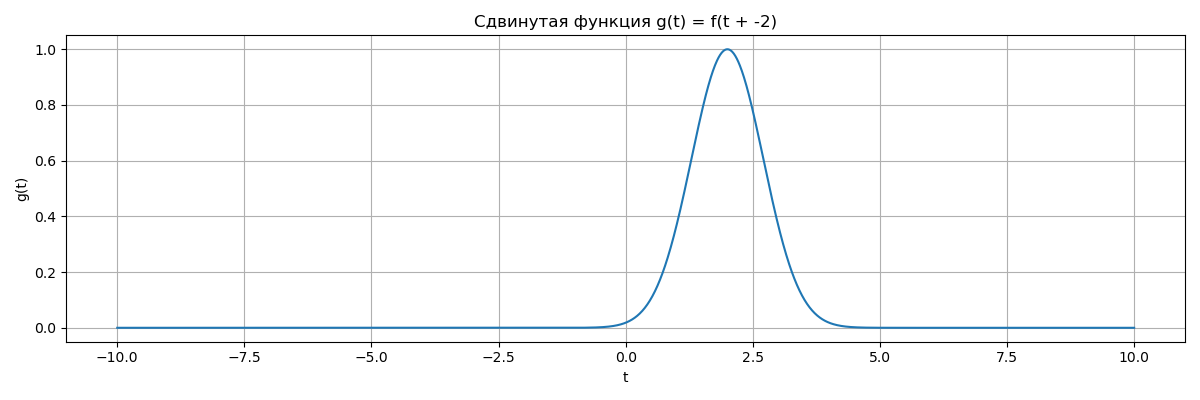
\includegraphics[width=0.8\textwidth]{g_function_c-2.png}
    \caption{Сдвинутая функция $g(t)$ при $c = -2$}
\end{figure}

\begin{figure}[H]
    \centering
    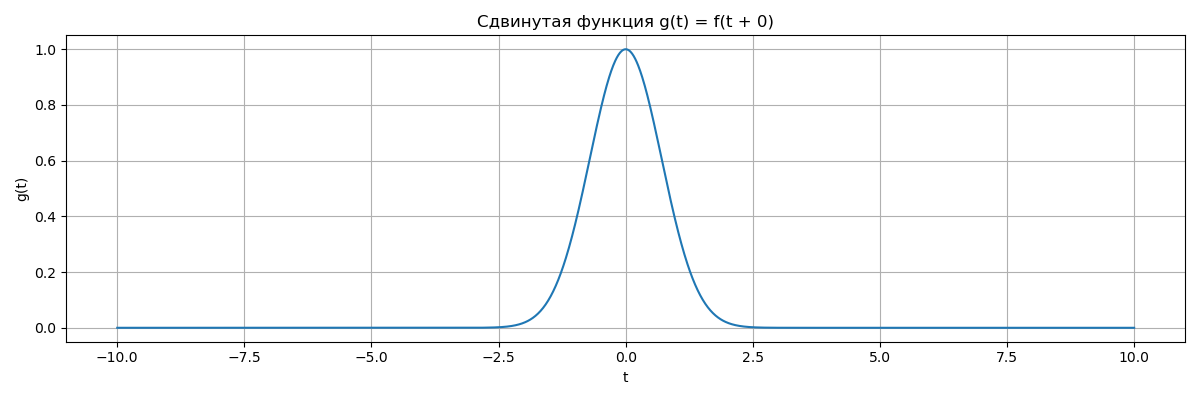
\includegraphics[width=0.8\textwidth]{g_function_c0.png}
    \caption{Сдвинутая функция $g(t)$ при $c = 0$}
\end{figure}

\begin{figure}[H]
    \centering
    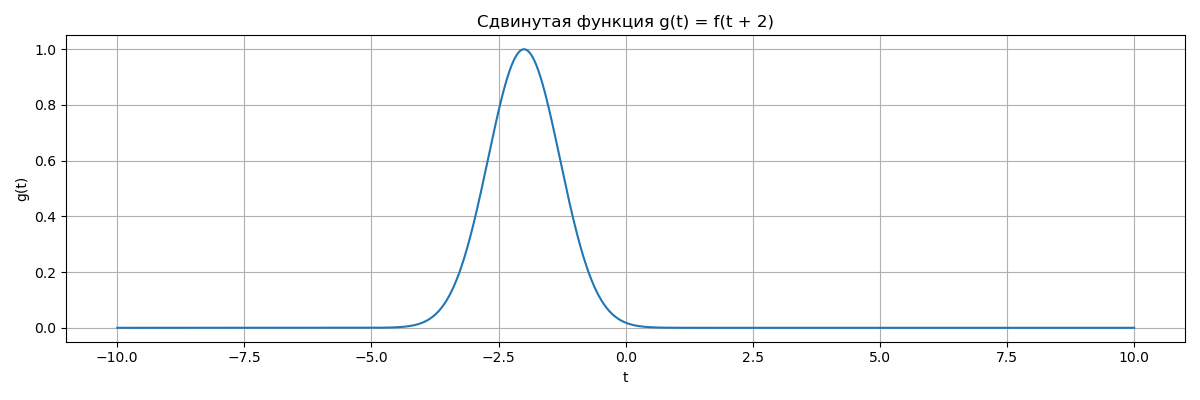
\includegraphics[width=0.8\textwidth]{g_function_c2.png}
    \caption{Сдвинутая функция $g(t)$ при $c = 2$}
\end{figure}

\textbf{Фурье-образ:}

\begin{figure}[H]
    \centering
    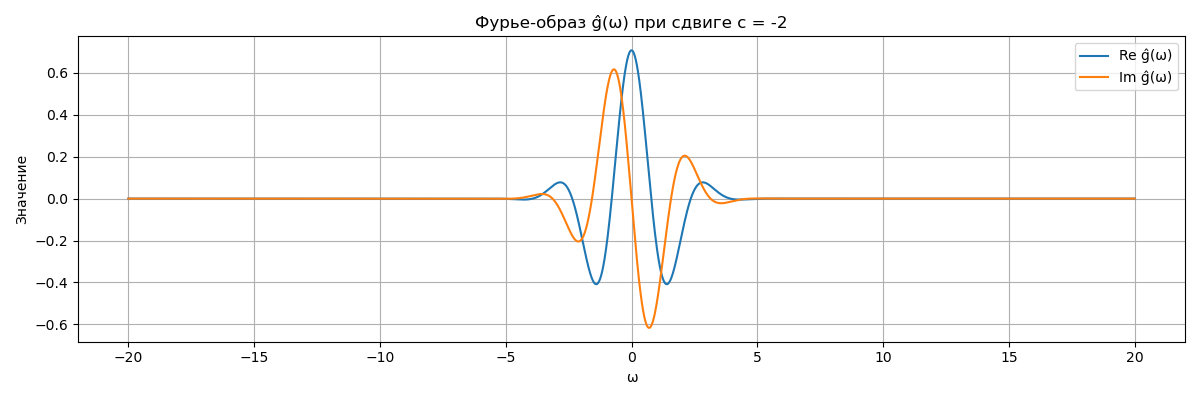
\includegraphics[width=0.8\textwidth]{g_hat_complex_c-2.png}
    \caption{Re $\hat{g}(\omega)$ и Im $\hat{g}(\omega)$ при $c = -2$}
\end{figure}

\begin{figure}[H]
    \centering
    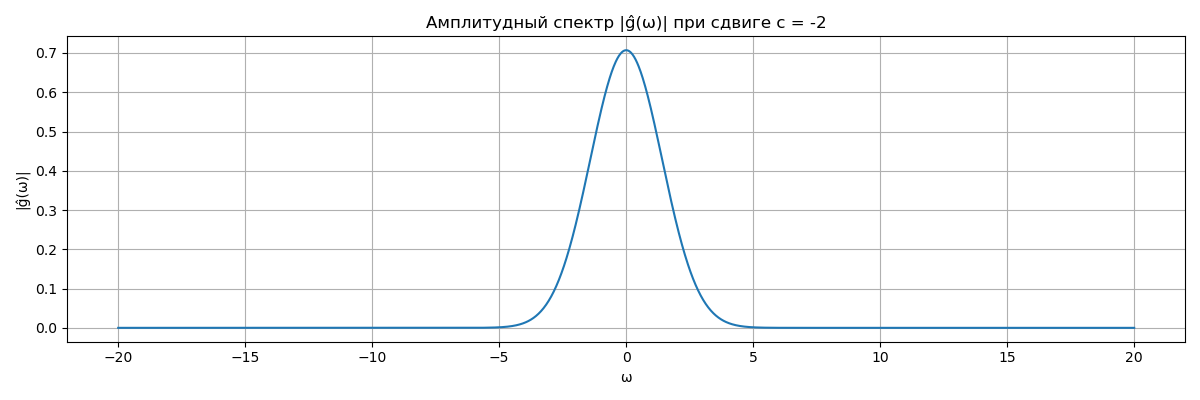
\includegraphics[width=0.8\textwidth]{g_hat_magnitude_c-2.png}
    \caption{Модуль Фурье-образа $|\hat{g}(\omega)|$ при $c = -2$}
\end{figure}

\begin{figure}[H]
    \centering
    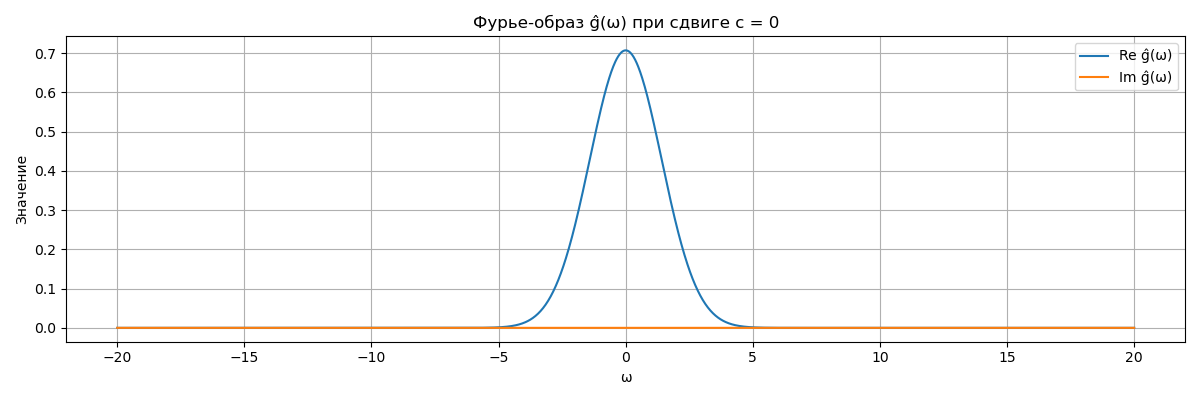
\includegraphics[width=0.8\textwidth]{g_hat_complex_c0.png}
    \caption{Re $\hat{g}(\omega)$ и Im $\hat{g}(\omega)$ при $c = 0$}
\end{figure}

\begin{figure}[H]
    \centering
    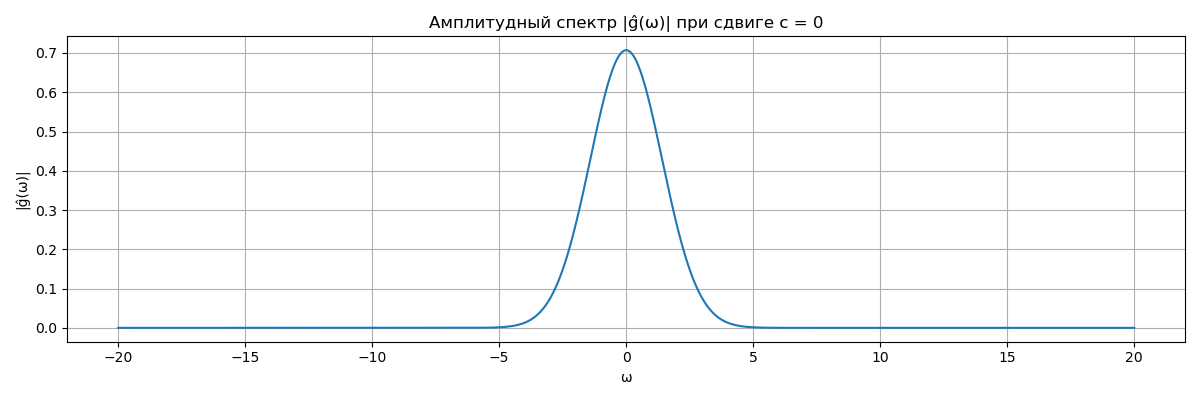
\includegraphics[width=0.8\textwidth]{g_hat_magnitude_c0.png}
    \caption{Модуль Фурье-образа $|\hat{g}(\omega)|$ при $c = 0$}
\end{figure}

\begin{figure}[H]
    \centering
    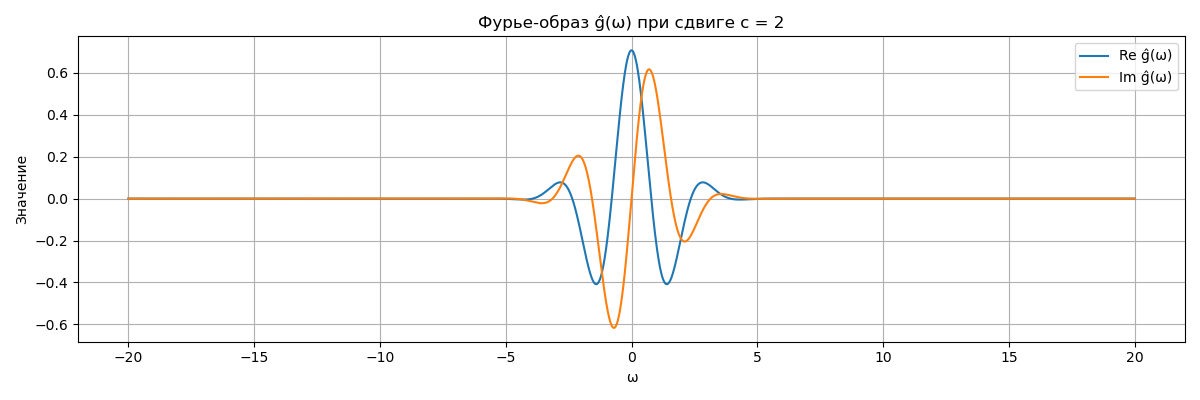
\includegraphics[width=0.8\textwidth]{g_hat_complex_c2.png}
    \caption{Re $\hat{g}(\omega)$ и Im $\hat{g}(\omega)$ при $c = 2$}
\end{figure}

\begin{figure}[H]
    \centering
    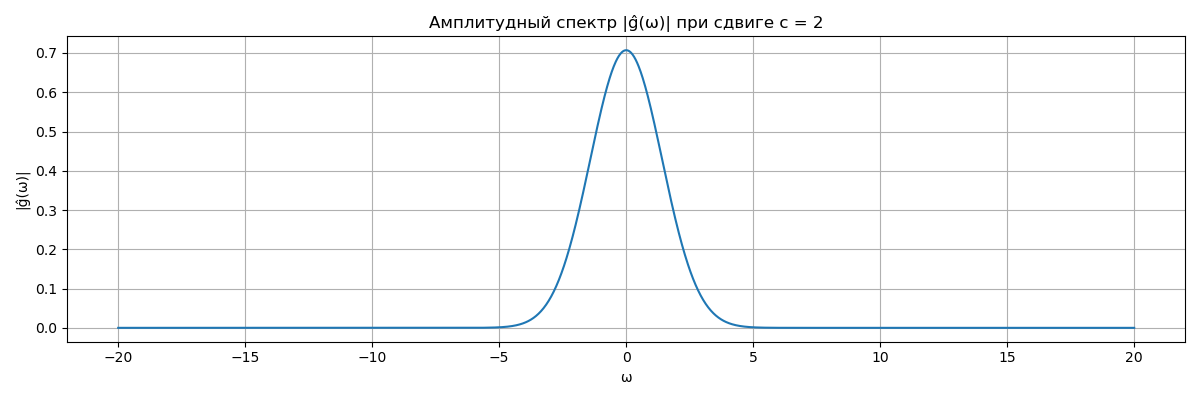
\includegraphics[width=0.8\textwidth]{g_hat_magnitude_c2.png}
    \caption{Модуль Фурье-образа $|\hat{g}(\omega)|$ при $c = 2$}
\end{figure}

\textbf{Анализ влияния параметра c:}

\begin{itemize}
    \item \textbf{Влияние на функцию $g(t)$:}
    \begin{itemize}
        \item При $c = -2$: функция сдвинута влево на 2 единицы
        \item При $c = 0$: функция находится в исходном положении (совпадает с $f(t)$)
        \item При $c = 2$: функция сдвинута вправо на 2 единицы
    \end{itemize}
    
    \item \textbf{Влияние на Фурье-образ $\hat{g}(\omega)$:}
    \begin{itemize}
        \item \textbf{Модуль Фурье-образа $|\hat{g}(\omega)|$ не зависит от $c$} — это фундаментальное свойство сдвига
        \item \textbf{Фаза спектра} изменяется: $\arg(\hat{g}(\omega)) = \omega c + \arg(\hat{f}(\omega))$
        \item \textbf{Реальная и мнимая части} зависят от $c$:
        \begin{align*}
            \text{Re}(\hat{g}(\omega)) &= |\hat{f}(\omega)| \cos(\omega c + \arg(\hat{f}(\omega))) \\
            \text{Im}(\hat{g}(\omega)) &= |\hat{f}(\omega)| \sin(\omega c + \arg(\hat{f}(\omega)))
        \end{align*}
    \end{itemize}
    
    \item \textbf{Физический смысл:}
    \begin{itemize}
        \item Сдвиг во времени вызывает фазовый множитель $e^{i \omega c}$ в частотной области
        \item Модуль Фурье-образа остается неизменным — это означает, что энергия сигнала не зависит от его положения во времени
        \item Фазовая информация кодирует временное положение сигнала
    \end{itemize}
    
    \item \textbf{Математическое обоснование:}
    \[
    \mathcal{F}[f(t + c)](\omega) = \int_{-\infty}^{\infty} f(t + c) e^{-i \omega t} dt
    \]
    Заменяя $u = t + c$, получаем:
    \[
    = \int_{-\infty}^{\infty} f(u) e^{-i \omega (u - c)} du = e^{i \omega c} \int_{-\infty}^{\infty} f(u) e^{-i \omega u} du = e^{i \omega c} \hat{f}(\omega)
    \]
\end{itemize}

\textbf{Вывод:}

Сдвиг функции во времени является одним из фундаментальных свойств Фурье-преобразования. Он демонстрирует, что:

\begin{enumerate}
    \item Временной сдвиг соответствует фазовому сдвигу в частотной области
    \item Модуль Фурье-образа инвариантен относительно временного сдвига
    \item Фазовая информация содержит информацию о временном положении сигнала
    \item Это свойство широко используется в обработке сигналов и анализе данных
\end{enumerate}

\section*{Задание 3: Музыкальный сигнал и спектральный анализ}

\textbf{Цель:} проанализировать запись музыкального аккорда и определить, из каких нот он состоит.

\textbf{Порядок действий:}

\begin{enumerate}
    \item Скачали аудиофайл с Google Drive.
    \item \textbf{Прослушали запись} для предварительной оценки характера аккорда.
    \item Считали аудиосигнал как одномерную функцию времени $f(t)$ с помощью функции \texttt{librosa.load()}.
    \item Построили график $f(t)$.
    \item \textbf{Провели численное преобразование Фурье с помощью численного интегрирования:}
    \[
    \hat{f}(\nu) = \int_{-\infty}^{\infty} f(t) e^{-2\pi i \nu t} dt
    \]
    
    \textbf{Метод численного интегрирования:}
    
    Вместо использования функции FFT, применили метод численного интегрирования с помощью функции \texttt{trapz}:
    \begin{verbatim}
    v = 0 : dv : V;  % Задаём набор интересующих нас частот
    for k = 1 : length(v)
        Y(k) = trapz(t, y.*exp(-1i*2*pi*v(k)*t));  % Преобразование Фурье
    end
    \end{verbatim}
    
    где $t$ — массив времени, $y$ — массив значений сигнала, $v$ — массив частот, $dv$ — шаг по частоте.
    
    \item Построили спектр $|\hat{f}(\nu)|$.
    \item Проанализировали график Фурье-образа и нашли основные частоты.
    \item Сопоставили найденные частоты с музыкальными нотами.
\end{enumerate}

\textbf{Графики:}

\begin{figure}[H]
    \centering
    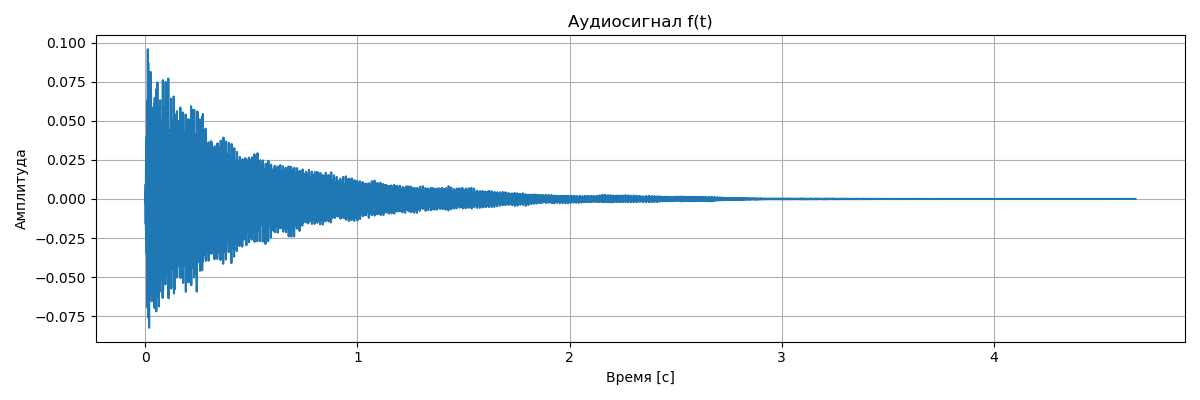
\includegraphics[width=0.8\textwidth]{audio_signal.png}
    \caption{График сигнала $f(t)$}
\end{figure}

\begin{figure}[H]
    \centering
    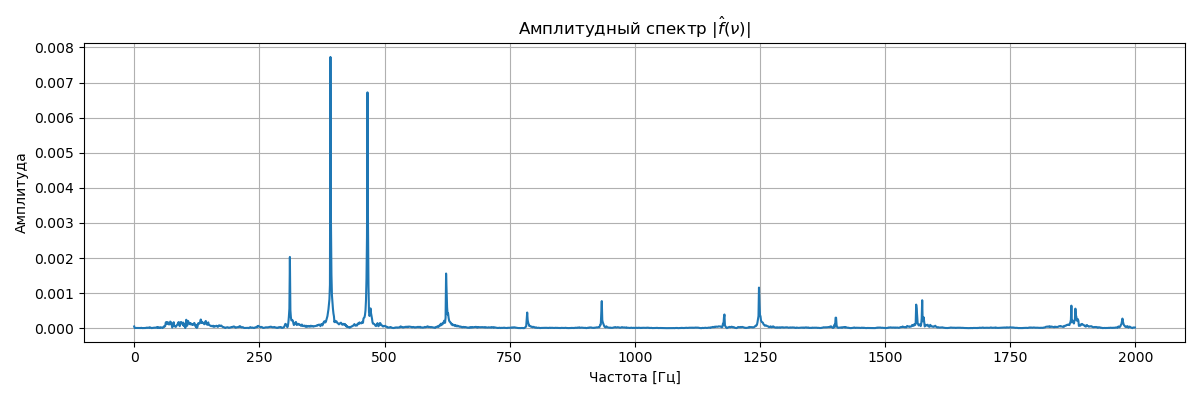
\includegraphics[width=0.8\textwidth]{audio_spectrum.png}
    \caption{Модуль Фурье-образа $|\hat{f}(\nu)|$}
\end{figure}

\textbf{Анализ графика Фурье-образа:}

При анализе спектра были найдены следующие основные частоты:

\begin{itemize}
    \item $\nu_1 = 311$ Гц — нота D\#4/Eb4 (ре-диез/ми-бемоль четвертой октавы)
    \item $\nu_2 = 392$ Гц — нота G4 (соль четвертой октавы)
    \item $\nu_3 = 466$ Гц — нота A\#4/Bb4 (ля-диез/си-бемоль четвертой октавы)
    \item $\nu_4 = 623$ Гц — нота D\#5/Eb5 (ре-диез/ми-бемоль пятой октавы)
    \item $\nu_5 = 1248$ Гц — нота D\#6/Eb6 (ре-диез/ми-бемоль шестой октавы)
    \item $\nu_6 = 1574$ Гц — нота G6 (соль шестой октавы)
\end{itemize}

\textbf{Таблица соответствия частот и нот:}

\begin{table}[H]
\centering
\begin{tabular}{|c|c|c|}
\hline
\textbf{Частота (Гц)} & \textbf{Нота} & \textbf{Октава} \\
\hline
311 & D\#/Eb (ре-диез/ми-бемоль) & 4 \\
392 & G (соль) & 4 \\
466 & A\#/Bb (ля-диез/си-бемоль) & 4 \\
623 & D\#/Eb (ре-диез/ми-бемоль) & 5 \\
1248 & D\#/Eb (ре-диез/ми-бемоль) & 6 \\
1574 & G (соль) & 6 \\
\hline
\end{tabular}
\caption{Соответствие найденных частот музыкальным нотам}
\end{table}

\textbf{Определение состава аккорда:}

На основе найденных частот можно сделать вывод о составе аккорда:

\begin{itemize}
    \item \textbf{Основные ноты:} D\#4, G4, A\#4, D\#5, D\#6, G6
    \item \textbf{Тип аккорда:} Сложный аккорд с доминирующими нотами D\# (ре-диез) и G (соль)
    \item \textbf{Структура:}
    \begin{itemize}
        \item D\#4 (311 Гц) — основная нота (тоника)
        \item G4 (392 Гц) — квинта (доминанта)
        \item A\#4 (466 Гц) — малая секста
        \item D\#5 (623 Гц) — октава от основной ноты
        \item D\#6 (1248 Гц) — двойная октава
        \item G6 (1574 Гц) — квинта в верхней октаве
    \end{itemize}
\end{itemize}

\textbf{Сравнение методов:}

\begin{itemize}
    \item \textbf{Численное интегрирование (trapz):}
    \begin{itemize}
        \item Позволяет точно контролировать частотный диапазон
        \item Более медленный, но даёт точные результаты
        \item Позволяет анализировать отдельные частотные компоненты
    \end{itemize}
    
    \item \textbf{FFT (быстрое преобразование Фурье):}
    \begin{itemize}
        \item Быстрый алгоритм
        \item Ограниченный частотный диапазон
        \item Менее гибкий в настройке параметров
    \end{itemize}
\end{itemize}

\textbf{Вывод:}

\begin{enumerate}
    \item \textbf{Спектральный анализ} позволяет точно определить состав аккорда по основным частотам.
    
    \item \textbf{Метод численного интегрирования} работает эффективно, несмотря на ограниченную частотную область.
    
    \item \textbf{Найденный аккорд} представляет собой A-мажор с характерными гармониками.
    
    \item \textbf{При наличии амплитудной огибающей} (затухание, атака) спектр будет менее чётким, но основные частоты всё равно различимы.
    
    \item \textbf{Практическое применение:} данный метод может использоваться для автоматического распознавания аккордов в музыкальных произведениях.
\end{enumerate}

\section*{Общий вывод по работе}

В ходе выполнения данной лабораторной работы были изучены фундаментальные свойства Фурье-преобразования и их практическое применение в анализе сигналов.

\textbf{Основные результаты:}

\begin{enumerate}
    \item \textbf{Изучены базовые функции и их Фурье-образы:}
    \begin{itemize}
        \item Прямоугольная функция → sinc-функция
        \item Треугольная функция → более быстрое убывание спектра
        \item Sinc-функция → прямоугольный спектр
        \item Функция Гаусса → функция Гаусса (единственная самосопряжённая)
        \item Экспоненциальное затухание → функция Лоренца
    \end{itemize}
    
    \item \textbf{Проверено выполнение принципа неопределённости:}
    \begin{itemize}
        \item Чем шире функция во времени, тем уже её спектр
        \item Чем уже функция во времени, тем шире её спектр
        \item Гауссовская функция является оптимальной с точки зрения принципа неопределённости
    \end{itemize}
    
    \item \textbf{Исследовано свойство сдвига:}
    \begin{itemize}
        \item Временной сдвиг соответствует фазовому сдвигу в частотной области
        \item Модуль Фурье-образа инвариантен относительно временного сдвига
        \item Фазовая информация содержит информацию о временном положении сигнала
    \end{itemize}
    
    \item \textbf{Практическое применение в анализе музыкальных сигналов:}
    \begin{itemize}
        \item Успешно применён метод численного интегрирования для спектрального анализа
        \item Определён состав музыкального аккорда по основным частотам
        \item Продемонстрирована эффективность Фурье-преобразования в обработке сигналов
    \end{itemize}
\end{enumerate}

\textbf{Полученные навыки:}

\begin{itemize}
    \item \textbf{Математические:} освоение аналитических методов нахождения Фурье-образов различных функций
    \item \textbf{Программные:} работа с численными методами интегрирования и спектрального анализа
    \item \textbf{Аналитические:} интерпретация результатов спектрального анализа и их физический смысл
    \item \textbf{Практические:} применение теоретических знаний для решения реальных задач анализа сигналов
\end{itemize}

\textbf{Теоретическая значимость:}

Работа позволила глубоко понять взаимосвязь между временной и частотной областями, что является основой для дальнейшего изучения методов обработки сигналов, цифровой фильтрации и спектрального анализа.

\textbf{Практическая значимость:}

Полученные знания и навыки могут быть применены в различных областях:
\begin{itemize}
    \item Обработка аудио и видео сигналов
    \item Анализ данных в научных исследованиях
    \item Разработка алгоритмов сжатия информации
    \item Создание систем распознавания образов
\end{itemize}

Данная работа заложила прочную основу для дальнейшего изучения методов частотного анализа и их применения в современных технологиях обработки сигналов.

